\section{driver}
The Panstamps' drivers were developed in C++. Each member in the network, namely serverNode, actuatorNode and sensorNode, has its own driver; nevertheless, all of them are based on the class "ccNode" as shown by the UML graph in Figure~\ref{fig:driverUML}. In other other words, ccServer, ccActuatorNode and ccSensorNode are all subclasses of the superclass "ccNode". 

All the nodes classes' names start with "cc" to denote that their communication depends completely on the class CC1101, which manages the transceiver integrated in each Panstamp.

\begin{figure}[h!] 
 \centering
 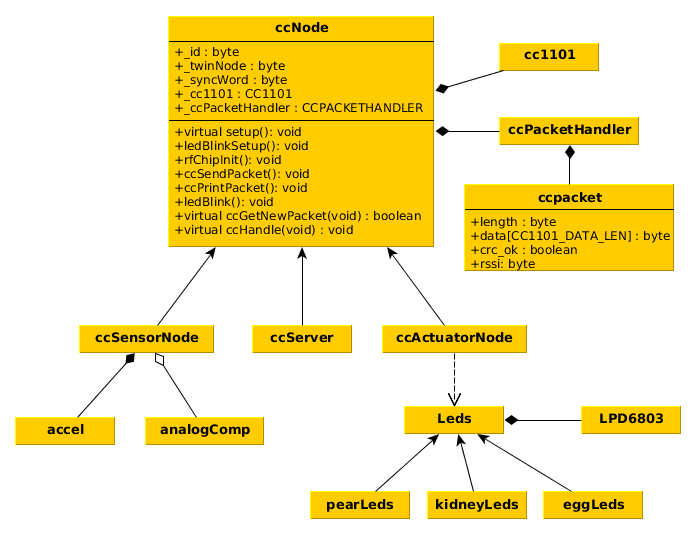
\includegraphics[width= 0.5\textwidth, clip=true,keepaspectratio=true] {./graph/driver-short.png}
 \caption{Driver's short UML }
 \label{fig:driverUML}
\end{figure}  

\subsection{ccpacket class}

The class ccpacket contains the backbone for all the messages (packages) shared by the network's nodes. As depicted in Figure~\ref{fig:driverUML}, this class' attributes are:
\begin{itemize}
\item length, which determines the size of each package
\item data, an array that holds the packet information
\item crc\_ok. This boolean value set by the transceiver, upon receiving a packet, indicates the packet's data integrity. 
\item rssi. This value is set by the CC1101 that receives the packet and indicates the received signal strength.
\end{itemize}

In our implementation, the packet's data length was set to 5 bytes. There are two types of packets:
\begin{itemize}
\item Notification packets
\item Command packets
\end{itemize}

\subsubsection{Notification packets}
\label{sec:Notification packet}
Notification packets can be sent by all nodes of the network; they inform other nodes about current events. 
For example, when a node is moved or kicked, it broadcasts a notification packet to all nodes to inform about this occurrence. 

Table~\ref{Notification-packet} shows Notification packet's structure:

\begin{table}[h]
  \centering
  \begin{tabular}{ c | c }
    \hline
    \textbf{Name} & \textbf{Value}\\ [0.5ex]    
    \hline
    Receiver Id & data[0] \\
    Sender Id & data[1] \\
    Admin Key & data[2]\\
    Near Node Id or Dummy & data[3]\\
    Dummy & data[4]\\      
    \hline
  \end{tabular}
  \caption[Notification packet]%
          {Notification packet}
  \label{Notification-packet}
\end{table}

Depending on the value of "Receiver Id", a message is received by all nodes or just by a single one. To broadcast, "Receiver Id" has to be set to "0" (zero). In other words, a packet is broadcasted when packet.data[0] is set to "0" (see \url{http://code.google.com/p/panstamp/wiki/LowLevelLibrary}).
When the packet has to be sent to just a single node, "Receiver id" holds the receiver node id.

The "Sender Id" indicates which node created and sent the packet. This data is important for interpreting any packet's meaning.

"Admin Key" points out an specific event perceived by a node in the network. When a notification packet is received by the server, this node creates a new Panstamp-to-Java server message (see section~\ref{sec:Panstamp-to-Java server message}) to inform the Java server about the new event. Notification packets share the same keys as the Panstamp-to-Java server messages; to see all possible values that "Admin Key" can take, please refer to Table~\ref{Admin Keys}. 

When a module is moved or kicked, its sensor node broadcasts a notification packet (with "Admin Key" equal to \emph{shake\_event} or to \emph{kick\_event}) that is received by the all sensor nodes and by the server node. Each sensor node compares the rssi of the received notification packet to a specific threshold to determine if the node that broadcasted the notification packet is near. When the rssi is strong enough, the sensor node sends a notification packet to the server node with "Admin Key" equal to \emph{Near\_Node\_Event}. In this Notification packet, data[3] contains the id of the sensor node that was detected to be near. For the rest of the Notification packets, data[3] doesn't contain any real data (is a dummy value). 

To keep the same length for all packets, the Notification packets has a dummy byte in his data array ("data[4]"). Nevertheless, this data byte contains real data in the Command packets. 

\subsubsection{Command packets}
Command packets are sent only by the server node to the actuator nodes. 	

Table~\ref{Command-packet} shows the Command packet structure: 

\begin{table}[h]
  \centering
  \begin{tabular}{ c | c }
    \hline
    \textbf{Name} & \textbf{Value}\\ [0.5ex]    
    \hline
    Receiver Id & data[0] \\
    Sender Id & data[1] \\
    Metakey & data[2]\\
    Color1  & data[3]\\
    Color2 & data[4]\\ 	 
    \hline
  \end{tabular}
  \caption[Command packet]%
          {Command packet}
  \label{Command-packet}
\end{table}

The two first fields, Receiver Id and Sender Id, are the same as the ones contained in the Notification packet section (see section~\ref{sec:Notification packet}). In a Command packet, the Sender Id byte will be always "1", the server Id, because only the server send Commands Packets.

"Metakey" indicates to the actuator node what pattern has to be displayed by the led strand. Table~\ref{Meta Keys} contains the patterns implemented in the system.

\begin{table}[h]
  \centering
  \begin{tabular}{ c | c }
    \hline
    \textbf{Name} & \textbf{Value}\\ [0.5ex]    
    \hline
    Blink & 0 \\
    Fade & 1 \\
    Rainbow & 2\\
    Leds On & 3\\
    Leds Off & 4\\ 
    Onestripe & 5\\
    Stripes & 6 \\
    \hline
  \end{tabular}
  \caption[Meta Keys]%
          {Meta Keys}
  \label{Meta Keys}
\end{table}

Most of the patterns displayed by the led strands have one or two colors. Fields "Color1" and "Color2" contain   keys that represent colors. The color pallet implemented in this system has 13 key colors but this pallet can be easily extended. 

\subsection{ccPacketHandler}
\label{sec:ccPacketHandler}
The ccPacketHandler class is in charge of managing the creation of packets and the access of data in received packets. For these tasks, the class contains the ccPacket class. 

\subsection{ccNode}
delivery and reception of packets
\subsubsection{ccNode methods}
As shown Figure~\ref{fig:driverUML}, this abstract class is the base for all node classes. The most important methods in this superclass are:
\begin{itemize}
\item virtual setup() sets the node's attributes depending on its type. See section~\ref{sec:ccNode-attributes} 
\item rfChipSetup() initializes and configures the CC1101 chip 
\item ccSendPacket() sends packets to other nodes in the network
\item ccGetNewPacket() receives packets from other nodes. Its implementation is different in each type of node.
\item ccHandle() interprets the data contained in a packet; therefore, its implementation varies among the nodes' types.
\end{itemize}

\subsubsection{ccNode attributes}
\label{sec:ccNode-attributes}
Every node in the network has the following attributes:
\begin{itemize}
\item \_id stores the node's id
\item \_twinNode has the id of the other node contained in the same module. For instance, in a sensor node this attribute is the id of the actuator node contained in the same module.
\item \_syncWord identifies the network. All nodes in our network share the same syncWord.  
\item \_cc1101 is an instance of the cc1101 class with which the cc1101 transceiver is controlled.
\item \_ccPacketHandler is an instance of the ccPacketHandler class (see section~\ref{sec:ccPacketHandler}).
\end{itemize}
                        
\subsection{ccSensorNode}
The ccSensorNode class creates and sends notification packets based on the information provided by the physical sensors, namely the accelerometer and the voltage monitoring circuit. Additionally, it creates and sends a notification packet when another module is really close. We consider that two modules are closed to each other when the distance between them is about 30 cm or less.

To perform its tasks, the ccSensorNode class uses the accel and analogComp classes as shown in Figure~\ref{fig:driverUML}.

\subsubsection{Accel class}
\label{sec:Accel class}
The accel class reads the signals given by the accelerometer and determines, according to specific thresholds, if a module was shaken or kicked. Since each module has a different mass, the acceleration produced by the same force varies among the modules. Therefore, when an instance of the accel class is created, two thresholds are required: shakenThreshold and kickedThreshold. In our system, these thresholds were estimated by sampling and averaging the acceleration data in each different module (pear, kidney and egg).

In section~\ref{sec:Accelerometer}, we mentioned that the accelerometer ADXL355 mounted in the board GY-61 has a bandwith of 50 Hz; i.e., its output signal has a frequency of 50 Hz. According to Nyquist–Shannon sampling theorem (see reference XXX), a band-limited signal can be reconstructed from a countable sequence of samples if the signal's bandwidth is no greater than half the sampling rate. Therefore, the accel class samples the accelerometer's signal at a frequency of 200 Hz (1 sample each 5 milliseconds). As a result, the analog-to-digital sampling frequency is 4 times the accelerometer's signal bandwidth, which is greater than two times the accelerometer's bandwidth. 

\subsubsection{AnalogComp class}
With the AnalogComp class, the panstamps' Analog Comparator module can be activated and configured to enable interruptions. As explained in section~\ref{sec:Voltage monitoring circuit}, in our implementation, the Analog Comparator triggers an interruption in the sensor node when the voltage on the pin AIN0 (digital pin D6) decreases below the voltage in pin AIN1 (digital pin D7). 

\subsection{ccServer class}
The ccServer class' main purpose is to enable the communication between the Java Server and the other network nodes. 

First, this class receives Notification packets sent by the sensor nodes and transfers the data contained in these packets to the Java Server. Messages transferred from the panstamp server to the Java server are explained in section~\ref{sec:Panstamp-to-Java server message}. 

Second, the ccServer class receives commands from the Java Server and creates Command packets accordingly to the corresponding actuator nodes. To see how the messages transferred from the Java server to the panstamp server are structured, please refer to section (this section is missing). 

\subsection{ccActuatorNode class}	
The ccActuatorNode class is in charge of receiving Command packets and of transferring the pattern data to the Leds class.  			

\subsection{Leds class}	
The Leds class controls the led strand connected to the actuator node. It receives pattern data from the ccActuatorNode class and reproduces the expected led pattern in the module. Since each module type has a different number and spatial distribution of leds, a subclass of the Led class was created for each type of module, namely pearLeds, kidneyLeds and eggLeds. 

\subsubsection{LPD6803 class}	
This class, published originally by ladyada in github \cite{lady_ada_LPD6803}, provides the methods for settting-up and for controlling each led in the led strands we used in our system. 





